% Source: graduate-coursework/Sp26/CSCE775/Project/proposal_asv_3/proposal3_asv.tex
% Description: MDP interaction cycle. At each timestep the policy maps the 87D state to a hybrid action (discrete mode + continuous parameters). The water environment simulator returns the next state and a composite reward signal.

\documentclass[border=4pt]{standalone}
\usepackage{amsmath,amssymb}
\usepackage{pgfplots}
\usepackage{tikz}
\usepackage{xcolor}
\pgfplotsset{compat=1.18}
\usetikzlibrary{positioning, arrows.meta, shapes.geometric, fit, calc, backgrounds, patterns, decorations.pathreplacing}

\definecolor{Garnet}{HTML}{73000A}
\definecolor{Atlantic}{HTML}{466A9F}
\definecolor{Congaree}{HTML}{1F414D}
\definecolor{Horseshoe}{HTML}{65780B}
\definecolor{Rose}{HTML}{CC2E40}
\definecolor{Honeycomb}{HTML}{A49137}
\definecolor{Black90}{HTML}{363636}
\definecolor{Black70}{HTML}{5C5C5C}
\definecolor{Black50}{HTML}{A2A2A2}
\definecolor{Black30}{HTML}{C7C7C7}
\definecolor{Black10}{HTML}{ECECEC}
\definecolor{WarmGrey}{HTML}{676156}


\begin{document}
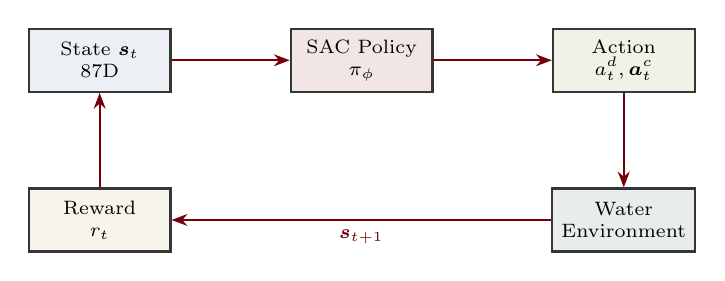
\begin{tikzpicture}[
    block/.style={draw=Black90, thick, minimum width=1.8cm, minimum height=0.8cm, align=center, font=\scriptsize},
    arr/.style={-{Stealth[length=2mm]}, thick, color=Garnet},
    every node/.style={font=\scriptsize}
]

\node[block, fill=Atlantic!10] (state) {State $\boldsymbol{s}_t$\\87D};
\node[block, fill=Garnet!10, right=1.5cm of state] (policy) {SAC Policy\\$\pi_\phi$};
\node[block, fill=Horseshoe!10, right=1.5cm of policy] (action) {Action\\$a^d_t, \boldsymbol{a}^c_t$};
\node[block, fill=Congaree!10, below=1.2cm of action] (env) {Water\\Environment};
\node[block, fill=Honeycomb!10, below=1.2cm of state] (reward) {Reward\\$r_t$};

\draw[arr] (state) -- (policy);
\draw[arr] (policy) -- (action);
\draw[arr] (action) -- (env);
\draw[arr] (env) -- node[below] {$\boldsymbol{s}_{t+1}$} (reward);
\draw[arr] (reward) -- (state);

\end{tikzpicture}
\end{document}
